\documentclass[11pt]{article}
\usepackage{graphicx}
\usepackage{float}

\begin{document}
	\title{Ticket Salad Coding Standards}
	\date{}
	\maketitle
	\newpage
	\tableofcontents
	\newpage
	
	\section{Introduction}
	\subsection{Purpose}
	The goal of these guidelines is to create uniform coding habits among software personnel in the
	engineering department so that reading, checking, and maintaining code written by different persons
	becomes easier. The intent of these standards is to define a natural style and consistency, yet leave
	to the authors of the engineering department source code, the freedom to practice their craft without
	unnecessary burden.
	
	
	\textbf{This document contains the coding standards that will be used in the TicketSalad system by the Hackermen team}
	\subsection{Scope}
	This document describes general software coding standards for code written by the Hackermen software team. It contains a class diagram and guidelines relating to different conventions and practices when coding.
	\section{System Design}
	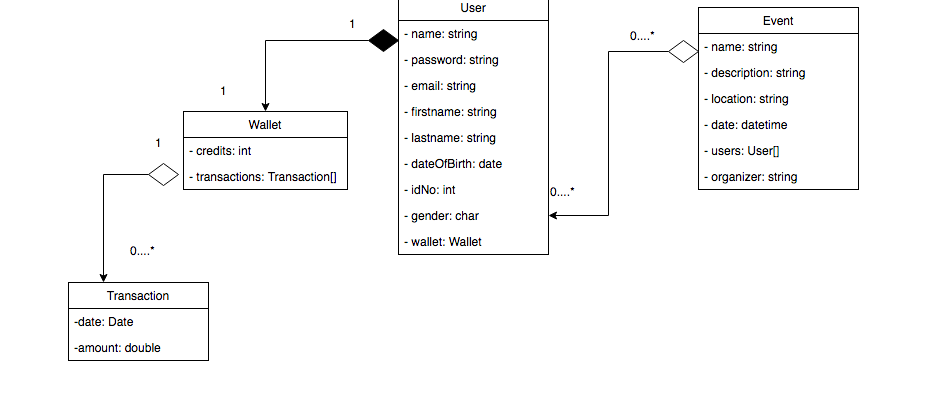
\includegraphics[scale=0.5]{Domain.png}
	\caption{\textbf{Figure 1:} A UML class diagram of the TicketSalad System}
	\section{Coding conventions}
	\subsection{Ensuring flexibility, reliability and efficiency}
	\subsubsection{Flexibility}
	The Hackermen team achieves flexible code, by writing code that is easily understood so that it can be easily modified. We achieved this by using identical naming and commenting conventions throughout all the software artefacts of the system thus ensuring a mutual understanding amongst the team of what functionality the code has and what it represents.
	\subsubsection{Reliability}
	The Hackermen team achieves reliable code, by writing code that does not allow for unexpected errors to produced while using the app, thus making the code reliable to use. We achieved this by ensuring that loops, start, end and iterate correctly, ensuring that no if statements are always true or always false ect.
	\subsubsection{Efficiency}
	The Hackermen team achieves efficient code by applying a modular practice to the code, thus making code more reusable and memory efficient. We achieve this by encapsulating different pieces of code with different functionalities allowing for the reuse of functions throughout all the code. 
	\subsection{Naming conventions}
	Naming conventions form a major part of coding standards as it makes code more readable by other developers thus increasing the scalability of the software.\textbf{The following file naming conventions will be used by the Hackerman team in the TicketSalad system}. "CamelCasing" us used for all naming scenarios.
	\subsubsection{File Names}
	Hackermen uses short file concise file names that describe the exact purpose of the file. E.g. The login html page will be called "Login.html".
	\subsubsection{Class Names}
	Hackermen uses short class names that are descriptive of the object that the class represent. E.g. A class representing the user will be called "User".
	\subsubsection{Function Names}
	Hackermen uses descriptive function names that describe the purpose of the code in the function. E.g. A function that contains the code to validate a password would be called "ValidatePassword".
	\subsubsection{Variable Names}
	Hackerman uses descriptive variable names that describe what information that the variable will store. E.g. A variable that stores a user's username would be called "userName".
	\subsection{Commenting practices}
	Commenting code eases the ability to understand complex code as there is a short description of the purpose of the code or any other information that needs to be noted. \textbf{Hackermen uses the following commenting practices in the TicketSalad System}
	
	Comments are only written on code that is not easy to interpret and understand by just reading the code. Comments will be written on functions that have more than one purpose and cannot be described entirely by the function name. E.g A function to login in the user will have a comment saying "Checks user input compare to database and returns a boolean". 
	
	Comments will also be used to describe complex algorithms and variables that are used in the code. 
	\subsection{Style conventions}
	The layout of code plays a large part in the ability for someone else to read the code as it allows for the readers ability to "flow" through the code to be improved because there is a logical layout.
	
	
	\textbf{The following style conventions will be used  by the Hackermen team in the TicketSalad system}
	\newpage
	\begin{itemize}
		\item Braces are each on a new line and the code inside the brace is indented to the right.
		\item Every statement is a new line.
		\item White blank lines will be used to break up large amounts of code into more easily understandable sections.
		\item There is no unnecessary white space.
	\end{itemize}
	\section{File structure}
	{The following file structure will be used  by the Hackermen team in the TicketSalad system}
	\begin{itemize}
		\item All Javascript (.js) files are stored in the controllers folder. JavaScript files are used to manipulate and change elements and values in HTML files and also manipulate the database.
		\item All CSS (.css) files are stored in the styles folder. CSS files are used to style the HTML files making.
		\item All HTML (.html) files are stored in the templates folder. HTML files contain the code for the interface that the user will be exposed to.
		\item All documentation (.pdf) files are stored in the documentation folder.
		
		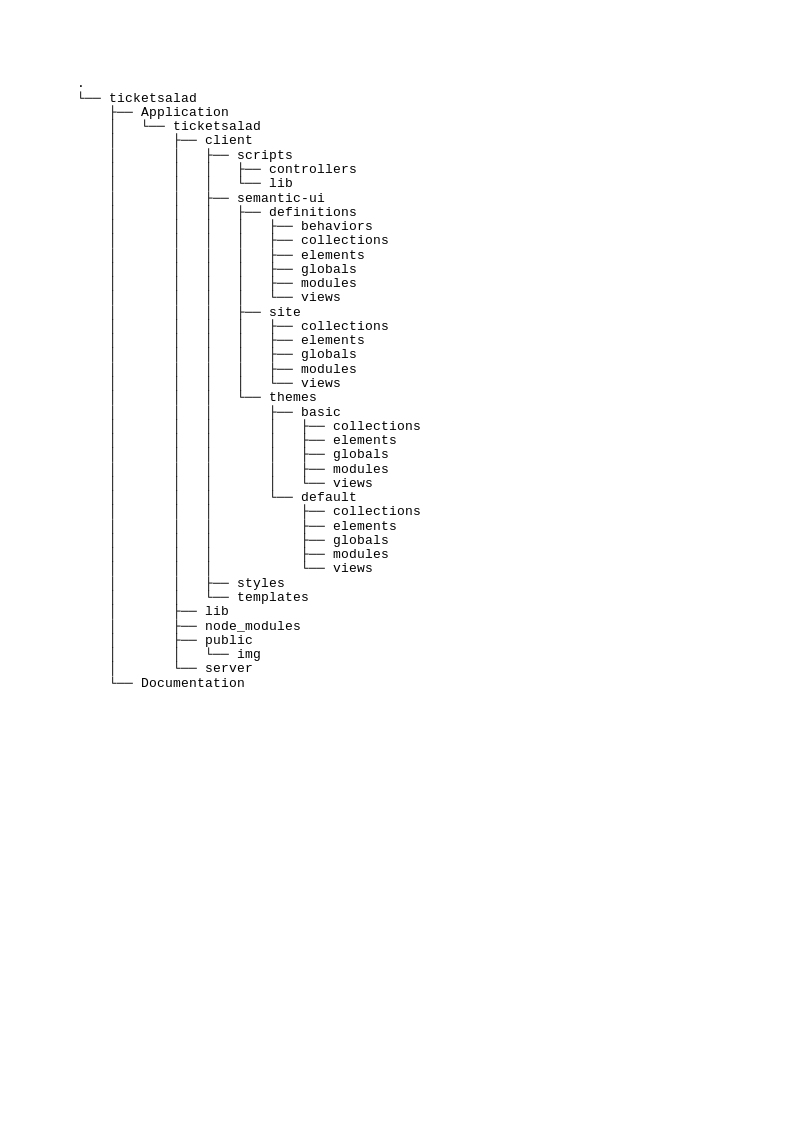
\includegraphics[scale=0.4]{tree}
		
		\caption{    \textbf{Figure 2:} A tree diagram of the TicketSalad file structure}
	\end{itemize}
	\newpage
	\section{Code Review practice}
	\subsection{Review Method}
	Upon creation of the Coding Standards the entire development team reviews the coding standards and present them to the stakeholders. If there is a concern it is raised and there is a discussion and if everyone agrees on the change a change is made.
	
	All code changes before a commit to the development branch are reviewed by code shepards Brandon Teixeira and Jarryd Baillie. The shepards will sit down with the changes and the Coding Standards document in front of them. The shepard will then ensure that all the coding requirements for that language is followed.
	
	\subsection{Application of coding standards}
	All files will have to comply to the coding standards including the testing files and structure.
	
	
	

	
	
	
\end{document}